% !TEX encoding = UTF-8
% !TEX TS-program = pdflatex
% !TEX root = ../tesi.tex

%**************************************************************
\chapter{Il progetto di stage}
In questo capitolo viene presentato il progetto di stage e le motivazioni della scelta.
\section{La piattaforma Zendesk}
\begin{figure}[!h] 
	\centering 
	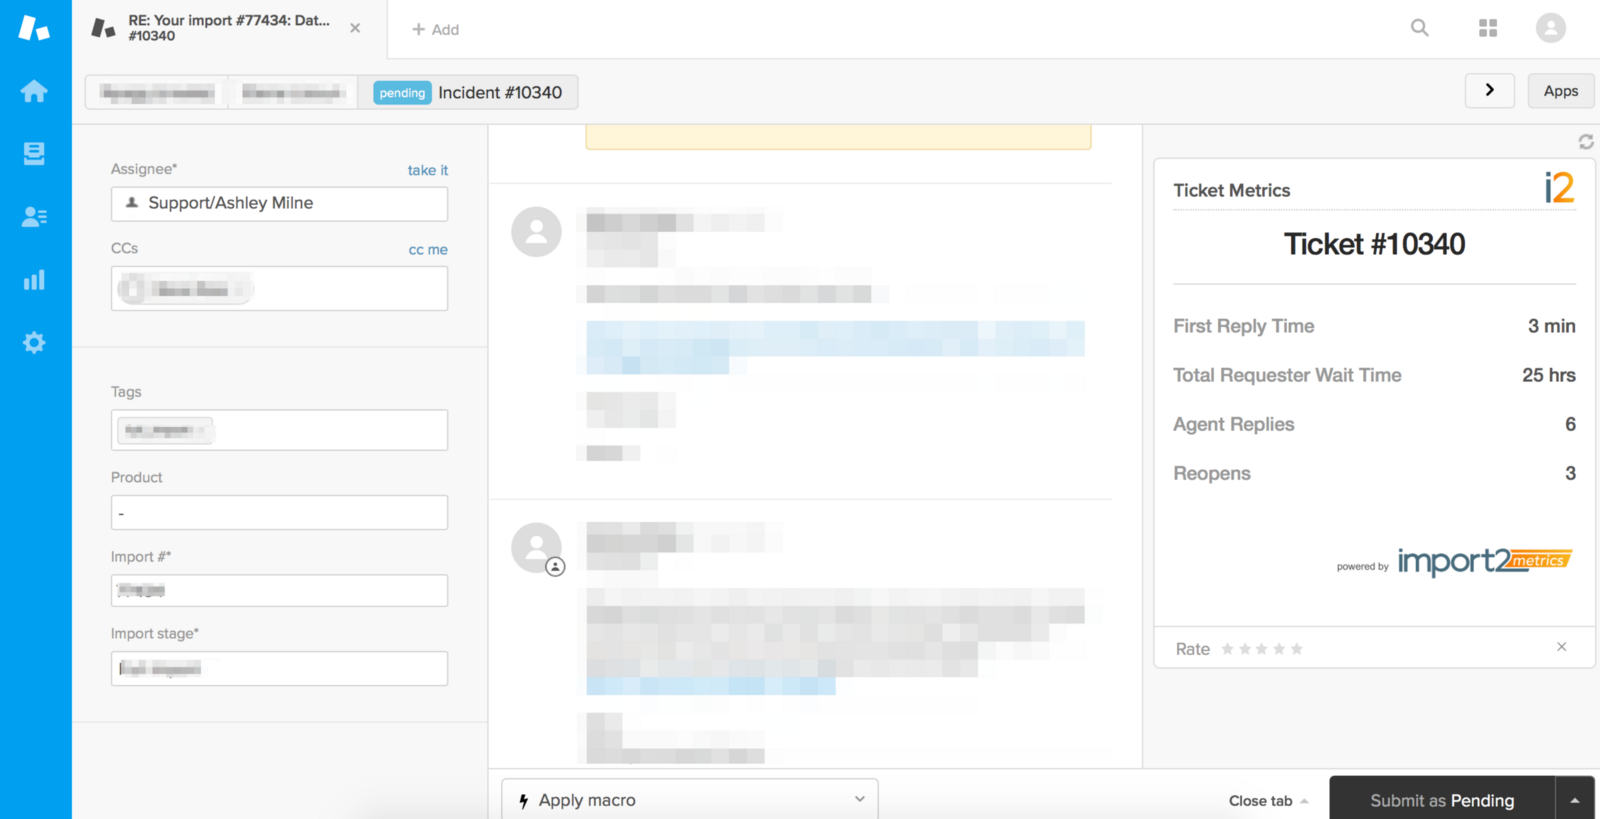
\includegraphics[width=0.8\columnwidth]{zendesk} 
	\caption{L'interfaccia utente Zendesk}
\end{figure}
Zendesk è una piattaforma online che permette a un'azienda di gestire le richieste provenienti da qualsiasi parte (mail, twitter, chat, ecc) dei proprio clienti in un unico posto sottoforma di tickets. E' la piattafroam più utilizzata nel mondo dalle aziende per quanto rigurada l'assitenza online. Il posto forte di questa piattaforma sta proprio nella sua semplicità. Presenta un'interfaccia molto userfrendly, dopo un paio di ore una persona prende completa confidenza con i strumenti da essa offerti. Gli utenti sono divisi in 2 cattegorie:
	\begin{itemize}
		\item Gli agenti: un agente si occupa di elaborare le richieste dei clienti. 
		\item Gli amministratori: un amministraore di Zendesk si occupa di gestire gli agenti e tutta la piattaforna. 
	\end{itemize}
\newpage
Zendesk inoltre offre ottimi strumenti per realizzare applicazioni esterne oppure integrarle nella piattaforma come app. Uno sviluppatore può realizzare una app di Zendesk utilizzando qualsiasi tecnologia web. L'applicazione realizzata può essere utilizzata sulla propria piattaforma come una app privata, oppure caricata nel marketplace di Zendesk a pagamento o gratuitamente.  
 
\begin{figure}[!h] 
	\centering 
	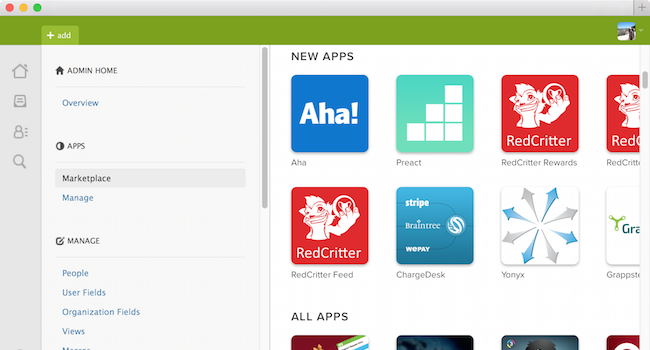
\includegraphics[width=0.8\columnwidth]{market} 
	\caption{Zendesk marketplace}
	\end{figure}

Il customer service via internet è un ambito sempre più in crescità, ci sono sempre più attività che si stanno spostando in internet. Un'attività di media dimenzione riceve al giorno in medai dai 500 a sopra le 1000 richieste dei clienti al giorno. La gestione con strumenti sbaglaiti di queste richieste può portare l'azienda a una notevole spesa(persona/lavoro) e soprattutto un feedback negativo dai clienti. 
\section{Lo stage}
Il progetto di stage è consistito principalmente nella realizzazione di una applicazione per la piattaforma di \emph{customer service} Zendesk. \\ L'applicazione realizzata permette agli agenti(persone che gestiscono le richieste dei clienti) e agli amministratori di Zendesk di realizzare contenuti(chiamati template) HTML e CSS in maniera molto semplice e veloce, ovvero utilizzando un editor \emph{drag-and-drop}. I template successivamente sono utilizzati nelle risposte verso i clienti. Questo permette di risparmiare una notevole quantità di tempo e non è necessario avere le conoscenze di HTML e CSS. Diverse aziende(clienti di Nextep) hanno fatta la richiesta esplicitamente di tale applicazione.
\\
\\
Alcuni dei benifici dell'applicazione CS-template:
\begin{itemize}
	\item realizzazione dei contenuti HTML e CSS senza sapere questi due linguaggi;
	\item la velocità con qui è possibile realizzare questi contenuti;
	\item permette agli agenti di realizzare le email predefinite, per rispondere alle richieste ricorrenti con un semplice click.
\end{itemize}
\newpage
\section{ Obiettivi dello stage}
Dopo una breve analisi insieme al tutor aziendale è sono stati definiti  seguenti obbietivi da raggiungere: 
\begin{itemize}
	\item apprendimento delle tecnologie necessarie per lo svolgimento del progetto;
	\item l'applicazione per la piattaforma Zendesk deve essere realizzata utilizzando Angular; 
	\item deve essere realizzata(sempre in Angular) anche una pagina degli \emph{admin} per la gestione di tutti i clienti che utilizzeranno tale applicazione;
	\item la pagina degli \emph{admin} deve essere accessibile solo dopo aver effettuato il \emph{login};
	\item il backend dell'applicazione deve essere tutto realizzato nei sistemi Cloud(AWS, Azure ecc.);
	\item tutta la progettazione deve essere documentata.
\end{itemize} 

\section{Motivazione della scelta}
